%% Template for a preprint Letter or Article for submission
%% to the journal Nature.
%% Written by Peter Czoschke, 26 February 2004
%%

\documentclass{nature}

%% make sure you have the nature.cls and naturemag.bst files where
%% LaTeX can find them
\usepackage{graphicx}	% Including figure files
\usepackage{amsmath}	% Advanced maths commands
\usepackage{amssymb}	% Extra maths symbols
%\usepackage{natbib}

\usepackage{hyperref}
\usepackage{url}
\usepackage{microtype}
\usepackage{rotating}
\usepackage{booktabs}
\usepackage{threeparttable}
\usepackage{tabularx}

\title{How and Why to run a Hack Week}

%% Notice placement of commas and superscripts and use of &
%% in the author list

\author{Daniela Huppenkothen, Anthony Arendt, David W. Hogg, Karthik Ram, Jake VanderPlas, Tal Yarkoni, \& Ariel Rokem}


\makeatletter
\let\saved@includegraphics\includegraphics
\AtBeginDocument{\let\includegraphics\saved@includegraphics}
\renewenvironment*{figure}{\@float{figure}}{\end@float}
\makeatother

\begin{document}

\maketitle

\begin{affiliations}
 \item UW Seattle
 \item NYU
 \item UC Berkeley
 \item UT Austin
\end{affiliations}

\begin{abstract}
Across almost all scientific disciplines, the instruments that record our experimental data and the methods required for storage and data analysis are rapidly increasing in complexity.
This gives rise to the need for scientific communities to adapt on shorter time scales than traditional university curricula allow for, and therefore requires new modes of knowledge transfer.
The universal applicability of data science tools to a broad range of problems has generated new opportunities to foster exchange of ideas and computational workflows across disciplines.
In recent years, hack weeks have emerged as an effective tool for fostering these exchanges by providing training in modern data analysis workflows.
While there are variations in hack week implementation, all events consist of a common core of three components: tutorials in state-of-the-art methodology, peer-learning and project work in a collaborative environment.
In this paper, we present the concept of a hack week in the larger context of scientific meetings and point out similarities and differences to traditional conferences.
We motivate the need for such an event and present in detail its strengths and challenges.
We find that hack weeks are successful at cultivating collaboration and the exchange of knowledge.
Participants self-report that these events help them both in their day-to-day research as well as their careers.
Based on our results, we conclude that hack weeks present an effective, easy-to-implement, fairly low-cost tool to positively impact data analysis literacy in academic disciplines, foster collaboration and cultivate best practices.
\end{abstract}

%\section*{}
\label{sec:introduction}
\dropcap{A}s data becomes cheaper to gather and store, research across a wide range of disciplines has become increasingly reliant on computational workflows involving a familiarity with aspects of statistical modeling, machine learning, scalable computation, and related skills. In addition, the recent reproducibility crises in several scientific fields has led to the growing realization that improving awareness of open science and reproducibility as well as practical skills in making research reproducible is essential to scientific progress \cite[e.g.][]{pashler2012,frye2015,gezelter2015,baker2016}.
Formal university curricula have been relatively slow to offer courses in these important topics: the slack in this area has often been picked-up by extra-curricular, ad-hoc efforts such as workshops (an overview and typography of such efforts in the data science context can be found in \cite{demasi2017}).
Well-known examples are the Software and Data Carpentry workshops providing training in research computing skills through a volunteer instructor program  \cite{b:wilson-swc-lessons-2016,teal2015data}.
At the same time, there has been a rise in the number of domain-specific courses focusing on statistics and computation within their field.
Examples include the \textit{Summer School in Statistics for Astronomers}\footnote{\url{http://astrostatistics.psu.edu/su16/}}, the Google Earth Engine User Summits\footnote{\url{https://events.withgoogle.com/google-earth-engine-user-summit-2017/}}, as well as a variety of project-focused (rather than pedagogical) meetings, such as the dotAstronomy meetings\footnote{\url{http://dotastronomy.com}}.
Shorter, but similar-spirit meetings have been held in conjunction with conferences, such as the Hack Days at the annual American Astronomical Society meetings, the Brainhack hackathons that take place in conjunction with meetings of the Organization for Human Brain Mapping and the Society for Neuroscience\cite{Cameron_Craddock2016-wc}, and a hackathon at the American Geophysical Union meeting\footnote{\url{http://onlinelibrary.wiley.com/doi/10.1002/2014EO480004/pdf}}.
Generally, pedagogically-focused events follow a classic academic model where novices learn new skills from experts, while project-focused workshops emphasize collaborative activities using existing skills.
A disadvantage of the pedagogical model is that it can tends to focus on a one-way flow of information from instructor to student, and can discount the potential contributions by students.
A disadvantage of the project model is the common perception that the week is designed for technical experts, which may discourage others from attending.
In 2014, we initiated an alternative model of ``Hack Weeks'' that try to fill the gaps between these models.
These are week-long events that combine pedagogy (often focused on statistical and computational techniques) together with time for hacks and creative projects, and with the goal of encouraging collaboration and learning among people at various stages of their career.

\begin{figure}
\begin{center}
\includegraphics[width=9cm]{fig/HackSpectrum}
\caption{Comparison of Extracurricular Workshop Models}
\label{fig:hackspectrum}
\end{center}
\end{figure}

As of the publication of this paper, we have run eight such hack week events: four focused on Astronomy, two focused on Neuroscience, and two focused on Geoscience.
Below we will share some of the philosophy behind the hack week model, results from surveys of participants, and practical lessons we have learned in organizing these events, as well as recommendations for future hack weeks in other disciplines (supplementary materials provide additional details on the practical aspects of organizing these events).

\section*{What is a hackathon?}

Hackathons are time-bounded, collaborative events that bring together participants around a shared challenge or learning objective \cite{Decker2015}.
Hackathons have historically focused on software development and technology design as a way to motivate innovation within industry.
In recent years, hackathons have expanded into a model for intensive short-term collaboration across disciplinary and topical boundaries.
In addition, because of their focus on participatory engagement, hackathons provide numerous opportunities to 'learn by doing' within a constructivist educational framework \cite{Bransford2000-lu,Papert1980-fh}.
With this in mind, hackathons around scientific topics, designed to foster collaboration \cite{Groen2015-cj,Moller2013-ah}, or provide an opportunity to learn \cite{Kienzler2015-zu,Lamers2014-xf}, are becoming more common.

%The recent surge in popularity of these events has resulted in a broad spectrum of ways to define the hackathon.
Following the typology of \cite{Drouhard2017}, we assert that core elements of all hackathons include opportunities for networking, the strengthening of social ties and the building of community connections, both within and across disciplines.
Building on these core elements, there are various implementations of the hackathon concept with respect to the overall purpose, mode of participation, style of work environment and motivation \cite{Drouhard2017}.
''Catalytic`` hackathons seek novel project ideas aimed at solving a tractable, well-defined challenge.
''Contributive`` hackathons seek to improve to an existing effort through focused work on discrete tasks, for example to make up for deficiencies in an ongoing project.
Finally, ''Communal`` hackathons place a strong focus on building a culture of practice and developing resources within an existing community, often defined by a specific domain of knowledge.

Our past hack week events most closely follow the communal hackathon model as it applies to scientific communities of practice.
Our approach aims to combine structured, tutorial-style instruction with informal education and peer learning opportunities occurring within projects and hacks.
Within the communal model we see these tools being implemented across a spectrum of approaches, the design of which depends on the specific characteristics of each community of practice (Figure 1).
For example, the astronomy community is relatively small and has a foundation of shared approaches and software implementations, allowing for a greater focus on project work over formal tutorials.
In contrast, both the neuro- and geoscience communities covered a broader range of sub-disciplines and had a less cohesive set of existing practices, calling for greater focus on tutorials and education.

We note that the terminology for these events is constantly evolving, and that the ''hackathon`` concept may have implicit connotations that are disfavored in some communities.
One criticism of hackathons is that they propel the ''geek`` stereotype and may present a barrier to creating an inclusive working environment, especially for women \cite{Decker2015}.
Another problem is the competitive atmosphere of many industry hackathons, where teams actively compete for prizes.
Because certain groups are more risk-averse than others, and risk-aversion traces demographics like gender, we urge caution when contemplating making an event competitive.
Other related nomenclature includes the ''unconference`` which is also a time-bounded event gathering together a specific community, but these often have minimal structure and do not necessarily have a focus on software.
The ''sprint`` or ''scrum`` label typically refers to an event focused on rapid software development on a specific set of code.
%This may be a component of our hack week model but it ignores the important pedagogical components.

\section*{Why run a Hack Week?}

There are several reasons to run a hack week of the sort described here.

\begin{itemize}
\item{\textit{Education and Training}: %Some hack weeks are more focused on education than others (see Figure 1).
While some hack weeks are focused more on education than others (Figure 1), there is often a skill-development component that entails extensive discussion on reproducible research and open science practices. Participants gain a strong foundation in open science practices from the diverse group setting and go on the become ambassadors for such practices in their respective fields. This type of lateral knowledge transfer is a core attribute of a hack week, and provides an opportunity to learn skills that are not described in papers and software implementations.}

\item{\textit{Tool Development}: Hack weeks present an opportunity for scientific software developers to meaningfully engage with users and critically evaluate applications to particular scientific issues.}

\item{\textit{Community Building}: Hack weeks provide a tremendous opportunity to catalyze community development through a shared interest in solving computational challenges with open source software. These events allow computationally minded researchers to break from the isolation of their academic departments and build connections and spark new collaborations.}


\item{\textit{Interdisciplinary research}: Intensive, time-bounded collaborative events are an excellent opportunity to experiment with concepts, questions, and methods that span boundaries within and across disciplines. Despite the fact that such interdisciplinary experiments are highly impactful \cite{Hall2012-hi}, they are often discouraged in risk averse traditional academia \footnote{\url{https://www.ncbi.nlm.nih.gov/labs/articles/12970550} and \url{https://www.researchgate.net/publication/8126355_EDUCATION_Risks_and_Rewards_of_an_Interdisciplinary_Research_Path}}.

\item{\textit{Recruitment and Networking}: Hack weeks are often a melting pot of participants from academia, government, and industry and provide numerous opportunities for networking. Close collaboration in diverse groups exposes skills that might be suitable for careers outside of one's narrow domain.}

\item{\textit{It's fun}: Hack weeks provide a respite from day-to-day research activities and provide a low-stress venue to learn new skills and attempt high-risk projects.}
\end{itemize}


It is worth noting that the reasons for participants to attend a hack week are as diverse as the goals that the organizing committee explicitly states.
This is largely a function of the diversity of the participants (see section below), and should be something that organizers design for.
Beginner participants may attend primarily to learn a new technique or method, while more experienced participants attend to gain more experience mentoring and teaching.
Some researchers may come with particular projects and collaborators in mind, while others come with a focus on learning and with no explicit plan for the project-based work.
%While it is very hard to design a workshop that is universally useful to all participants, in practice many researchers attend with the understanding that some components will be more congruent with their own goals than others, but also bring an open mind and a willingness to learn.
%In addition, the diversity of goals can effectively be a strength of the workshop, if the organizers can facilitate matching up participants with complementary goals.

\section*{Audience and Participant Selection}

Because hack weeks are at their core non-traditional workshops, it is worth thinking in detail about the target audience for a hack week, along with methods to select an appropriate group of participants. Here, appropriate essentially refers to 'most likely to achieve the stated goal of the hack week', though measuring that achievement remains a difficult issue itself.
This is especially important because hack weeks are very participant-driven workshops.
%At a traditional conference or summer school, the program will be largely set in advance by the organizing committee using the careful selection of speakers and lecturers.
%At a hack week much of the program is in flux both before and during the workshop.
In this context, a successful hack week requires participants who are both interested in participation and feel comfortable participating in discussions and taking risks.
Therefore, a robust, effective participant selection procedure is of crucial importance to the outcomes of the hack week and may require both careful engineering and an in-depth discussion among the organizers.

Perhaps unsurprisingly, the target audience for a hack week depends directly on the stated goal of the workshop.
At conferences, researchers typically report recent results to the community and network with other scientists largely from their discipline, leading to a fairly narrow target distribution in academic seniority and represented fields.
At a summer school, the aim is generally for senior researchers to transfer knowledge about a particular subject or field to novice researchers, primarily graduate students and early postdoctoral fellows.
Hack weeks differ in that knowledge transfer occurs across many levels of seniority, due to the relative newness of the content and the distributed knowledge base.
%Because the potential for knowledge transfer and community building is highest when the group is heterogeneous, participant diverse in both academic background and geographic location should be selected.
%This increases the chances that participants will take their newfound knowledge into their respective communities and spread it further.

Aside from these broad considerations, the tuning of the audience and participant selection will depend directly on several of the axes described in detail above.
In particular, education-focused workshops might be more homogeneous than project-focused workshops, and similarly single-discipline hack weeks may be more homogeneous than interdisciplinary ones.
Additional goals may be not directly related to the workshop itself, but on higher-order goals (e.g.\ increasing minority participation, knowledge transfer between academia and industry) that a community might find desirable and that can be directly addressed by engineering the participant selection.
% For example, women are still a small minority in computational astrophysics.
%One goal of a hack week could be to increase the participation of gender minorities in computation-focused research.
%Similarly, if a particular sub-field within a discipline is ahead of others in their computational approaches, it might be worthwhile to engineer the mix of participants such that a number of experts from that sub-field are present.
%One interesting axis to consider is the mix of academics versus participants from industry.
%The latter may often be more focused on practically useful applications of methods and data sets, and can therefore provide an important counterpoint to more theory-focused academics.
%In particular in fields where the career path from academia to industry is less immediately obvious (as this the case e.g. in astronomy, where little directly relevant industry exists), inviting back participants who transitioned to industry successfully can provide important role models and networking opportunities for junior participants.
%Finally, with much of data science currently performed in the private sector, industry participants can bring directly relevant knowledge and new scientific approaches to the table.

The need to carefully select participants dovetails with another requirement: transparency.
%Up to date, all hack weeks we have organized have been oversubscribed by at least a factor of two, and thus necessarily require turning applicants away.
The selection procedure should be as transparent to the applicants as possible, and the organizing committee should be held accountable for their performance.
Transparency is necessary for applicants to understand acceptance/rejection decisions, and accountability is of crucial importance for the detection of inherent biases in the selection, which may harm both the workshop's success as well as the larger community.

In order to maximize transparency in our selection process we are working to remove the human element from the decision making as far as possible and transfer some of these tasks to a well-designed algorithm.
Here, well-designed refers to several properties: (1) it is interpretable, i.e. the algorithm, its parameters and outputs can be understood by humans, (2) it is openly available, and thus the decision process can be inspected, (3) the algorithm itself does not perpetuate intrinsic biases in the data (though we will show below that an algorithm itself does not entirely remove the requirement of humans to be aware of their biases).

In practice, most selection procedures follow two separate steps, though in the case of human committees, these steps are often conflated.
In the first step, the merit of a candidate must be assessed: does the candidate fulfill the requirements posed by the goals of the workshop? %For example, at Astro Hack Week, it may be unrealistic to admit an undergraduate student in biochemistry, unless they had a compelling reason for attending.
This first step is difficult to automate, because it requires judgment calls, often based on long-form answers.
In the past, we have performed this step by blinding ourselves to a candidate's other attributes (including name and other personal information), and assess their candidacy based solely upon key questions asked specifically for this purpose.
When doing this procedure for a large enough sample, it is unlikely that the resulting pool of acceptable candidates is smaller than the number of available spaces at the workshop.
The second step in the selection procedure thus requires tie-breaking between equally acceptable candidates.
It is here where one may impose outside constraints on the selection based on the goals of the workshop.
If multiple competing constraints are considered, this task essentially becomes a complex optimization problem, for which algorithms exist that will outperform any human selection procedure.

In particular, the software \textit{entrofy}\footnote{\url{http://github.com/dhuppenkothen/entrofy}} employs one such algorithm and is capable of efficient selection of an optimal candidate set based on human target fractions.
It is worth noting that this algorithm is vulnerable toward biases in two ways: firstly, humans will set the target fractions for any category of interest.
If these targets reproduce the distribution of the overall sample of candidates, the selection will become essentially random.
Any human biases involved in setting these target fractions will be perpetuated in the selection procedure.
Secondly, perhaps more obviously, the algorithm can only act on information that has been collected.
Biased participant sets may still result from selection procedures that fail to include crucial categories (for example, it would be difficult to produce a student-heavy participant set for a summer school if the algorithm has no information about academic seniority).

%Within our hack weeks the goal of the selection procedure has always been diversity among several axes.
%This includes academic subdiscipline, to allow for maximally possible knowledge exchange between different domain fields, as well as with researchers from adjacent fields including statistics, computer science and data science.
%Other important categories revolve around the participants' previous knowledge in terms of machine learning, statistics and programming.
%Unlike for a summer school, we have generally selected for a diverse set of participants in order to be able to efficiently pair up novices and experts in projects.
%Finally, we also include demographic information with two main goals: firstly, representation has been proven to be an effective way to foster an inclusive environment where minority participants feel comfortable to participate and take risks.
%Secondly, we would like to boost the participation of minority researchers in computational astrophysics, and our hack week model provides a useful framework for doing so.

\section*{Themes}

To date, all organized hack weeks have been subject-specific.
That is, they aimed to bring together a community with a shared scientific interest, e.g.\ neuroscience, astronomy or geoscience.
This has several clear advantages.
In particular, communities organized by subject generally share the same language.%, which drastically cuts down on the time participants spend simply agreeing on scientific terms.
Similarly, the scientific objectives and questions are broadly clear to all participants.%: there is little need to explain in detail why a particular question may be of interest to the field.
Finally, there are practical considerations: while even within fields the use of particular data sets and software packages may differ quite widely, there is generally a shared understanding of the type of data usually taken, and the most common ways to analyze this data.
This leaves more time for active collaboration on cutting-edge science.

However, there are also drawbacks to limiting the theme of a hack week to a single field.
Homogeneity may be a disadvantage if it leads to \textit{group think} and inhibits new, creative solutions.
Within a field, the chance of participants being familiar with each other may be larger, leading to the formation of cliques and insufficient mixing.
These disadvantages may be mitigated by organizing a hack week around a technique (e.g. Gaussian Processes) or modality (e.g. imaging) instead.
In these case, building a shared vocabulary and understanding the major data analysis problems in each field is a crucial task.%, and should be allocated sufficient time in form of introductory talks or tutorials to foster cross-disciplinary collaboration.
On the other hand, cross-disciplinary hack weeks around a specific technique or type of data set allow methods developed in a specific field to diffuse into other subjects and therefore help avoid duplication of method development efforts.

An example of such events are the ImageXD (image processing across domains\footnote{\url{http://http://www.imagexd.org/}} meetings held at the UC Berkeley Institute for Data Science in the Summer 2016, and at the UW eScience Institute in the Spring of 2017.
These three-day events also included a mix of tutorials, talks, and joint work on projects, but in contrast to the hack weeks described in the present paper, these events included participants from a variety of different research fields, with the common thread being that they all have an interest in the analysis of images, as part their research.
%Thus, audience and speakers included researchers from wide array of domains: astronomy, neuroscience and geosciences, but also material science, chemistry, biology, medicine, engineering, and others.
%In addition, participants included computer vision researchers, who develop algorithms that can be applied to answer scientific questions.
%Similarly, a series of events at UC Berkeley (Text XD) focused on the analysis of text data across different domains of research.

\section*{Design considerations}

Design considerations depend very strongly on goals.
In general, longer events allow for a larger taught component, more ambitious projects and especially for cross-disciplinary events are more likely to provide enough time for different groups to effectively communicate across barriers of professional terminology.
On the other hand, because of their large participatory component, hack weeks tend to be exhausting, and long events may lead to fatigue among attendees, where active participation and measurable outcomes may drop sharply in the latter days of the workshops.
%This is particularly important if---as is often the case---participants continue participating in workshop-relevant activities even after the official component ends for the day.
Ways to mitigate these effects include capping taught components during the day, providing a reasonable clear schedule, and limiting parallel components to avoid decision fatigue.
%At Astro Hack Week, we have limited the scheduled taught components to no more than three out of nine hours for each of the five workshop days, and unscheduled (shorter) tutorials to a maximum of two per day.
%Even so, in our surveys, participants occasionally report concerns about choosing to attend tutorials versus working on projects.

Aside from time, space plays a particularly important role in facilitating a successful hack week.
Universities in general provide a convenient venue with existing structures to facilitate hack weeks (e.g. access to scientific publications, institutional support including staff and funding).
On the other hand, most spaces in universities are designed for lectures, which are diametrically opposed to unconference-style events.
Thus, finding an appropriate physical space within a university may be a challenge.
However, with the rise of active learning as a preferred teaching methods, traditional lecture spaces are transforming into more flexible spaces that are generally appropriate for hack weeks.
As a general rule, the smaller a hack week's emphasis on a taught component, the more flexible the space has to be, with ample opportunity for re-configuration.
%At Astro Hack Week, we have found it beneficial to spend one day mid-week at a different location (e.g. a company headquarter) to engage participants and break the routine.
%It is worth noting that collaborative spaces for non-traditional workshops are becoming more prevalent in academia (some attached to universities, some not) and may provide support and infrastructure that a traditional university location may not.

Another important design consideration is group size.
%With all previous hack weeks severely oversubscribed, it seems natural to simply admit more participants.
%However, this can counter the ideals of the workshop, in particular when building a community is one of its stated goals.
If the group is too large, participants are unlikely to even meet each other, and workshop cohesion may be lost as the workshop fractures into smaller groups, often among participants who already know each other.
This may inhibit knowledge transfer by clustering participants into small in-groups.
%Additionally, it is likely that the number participant-led components in the schedule may increase with workshop size.
%While generally desirable, a programme that is too crowded may lead to fatigue
On the other hand, if the size of the workshop is too small, it is unlikely to achieve the desired diversity among participants to foster new collaborations across sub-fields and disciplines.
In the past, we have found groups with sizes between 50 and 70 participants to be large enough to encourage a breadth of projects while allowing the workshop to function as a cohesive group.

As mentioned above, the balance between pedagogy and working depends both on the goals of the workshop and the topics around which the workshop is organized.
If participants have little shared knowledge, more teaching may be necessary in order to allow participants to effectively communicate with each other.
In communities where a shared understanding exists, tutorials can focus on more advanced or innovative topics, and less time may be allocated for them, leaving more time for active participation.
%In astronomy, a relatively small field, even students generally share a common knowledge base and have rudimentary knowledge about the types of data used and the challenges associated with each.
%Thus, we have focused the taught component of Astro Hack Week less on domain-specific knowledge, and instead offered tutorials in topics from domain-adjacent fields like statistics and computer science that attendees are unlikely to have encountered in their regular education.

Hack week outcomes, in turn, depend strongly on participants and are often a function of their interests and seniority.
some attendees arrive with the stated goal of writing a specific scientific article, usually more advanced participants with significant pre-knowledge of both hackathons and their topic of interest.
Many attendees arrive with the plan to learn a specific topic (such as machine learning) or bring a specific data set they believe the new knowledge may be applicable to.
This leads to a wide variety of project types from sandbox-style explorations to focused work efforts.
%It is worth noting that while a scientific paper need not be the stated goal of a hack (and is unlikely to be completed in the short time allocated in any case), results may still be published as short reports or unconference proceedings.
%For example, Neurohack week provides a venue for participants to publish a short (two-page) ''project report`` summarizing the hack that participants did during the week of NHW.
%Similarly, Python in Astronomy gathers all documents produced during the workshop (unconference transcripts, talk summaries, descriptions of sprint and hack projects) into citeable unconference proceedings.

\subsection*{Box 1: Impostor Syndrome}

The \textit{impostor phenomenon}, or \textit{impostor syndrome} (IS) is a dissonant feeling experienced by certain high-achieving individuals, that despite objective evidence to the contrary, they are in fact not as intelligent or capable as they appear.
Individuals with IS thus experience a fear of being ''found out``, shamed and expelled from their environment \cite{Clance1978-ef}.
Initial observations of the first Astro Hack Week conducted by data science ethnographer Brittany Fiore-Gartland\footnote{\url{http://astrohack week.org/blog/ethnographic-notes.html}} suggested that hack weeks are an environment prone to a particular kind of IS: participants might feel the need to be experts in multiple aspects of the activities pursued during a hack week: expertise in a scientific domain, as well as expertise in a the variety of technical tools used.
This particular form of IS hinges to some degree on the design focus on diversity of backgrounds (everyone else seems to know something that you do not!) and might be further exacerbated by the expectation that attendants expose their ideas to public scrutiny, find collaborators in a very short amount of time, and not least produce and present a successful hack at the end of the week\footnote{see also this insightful blog post: \url{https://medium.com/astronomy-without-stars/the-horror-of-hack-days-52c6b52cfc3b}}.
The prevalence of IS at a hack week may be endemic to the format, and should thus be a major concern for any organizing committee.
This is because of the chilling effect it tends to have on participants and the community as a whole, and particularly on women (in particular in fields in which women are under-represented) and members of ethnic and racial minorities, correlating with anxiety and other forms of mental distress \cite{Parkman2016-ro}.
Less severely, another major concern is that IS inhibits risk taking: participants experiencing it will be less likely to ask a question, to put forward an idea for a hack, to be pro-active about forming new collaborations.
 Many of the goals of a hack week, including the successful completion of projects, lateral knowledge transfer, as well as community building are hampered.
We are working within our hack weeks to mitigate IS using various techniques.
With respect to minority participants, ensuring adequate representation can decrease feelings of otherness and may help reduce IS.
More generally, being open about the presence and prevalence of IS can help participants feel more at ease.%(e.g. one Astro Hack Week participant remarked in a survey, \textit{''I really appreciated the direct acknowledgement of impostor syndrome on the first day.
%I think it helped ease the feeling!!``}).
Additionally, role models are very effective at encouraging positive behaviour: asking participants with prior experience at hack weeks at all academic levels to ask questions, even when they might know the answer, can help foster an inclusive environment that rewards risk taking.

\section*{Results}

\begin{figure*}[h!]
%\begin{center}
\begin{subfigure}[t]{\textwidth}
\centering
\caption{}
\includegraphics[width=11cm]{fig/eval_techskills.eps}
\end{subfigure}

\begin{subfigure}[t]{\textwidth}
\centering
\caption{}
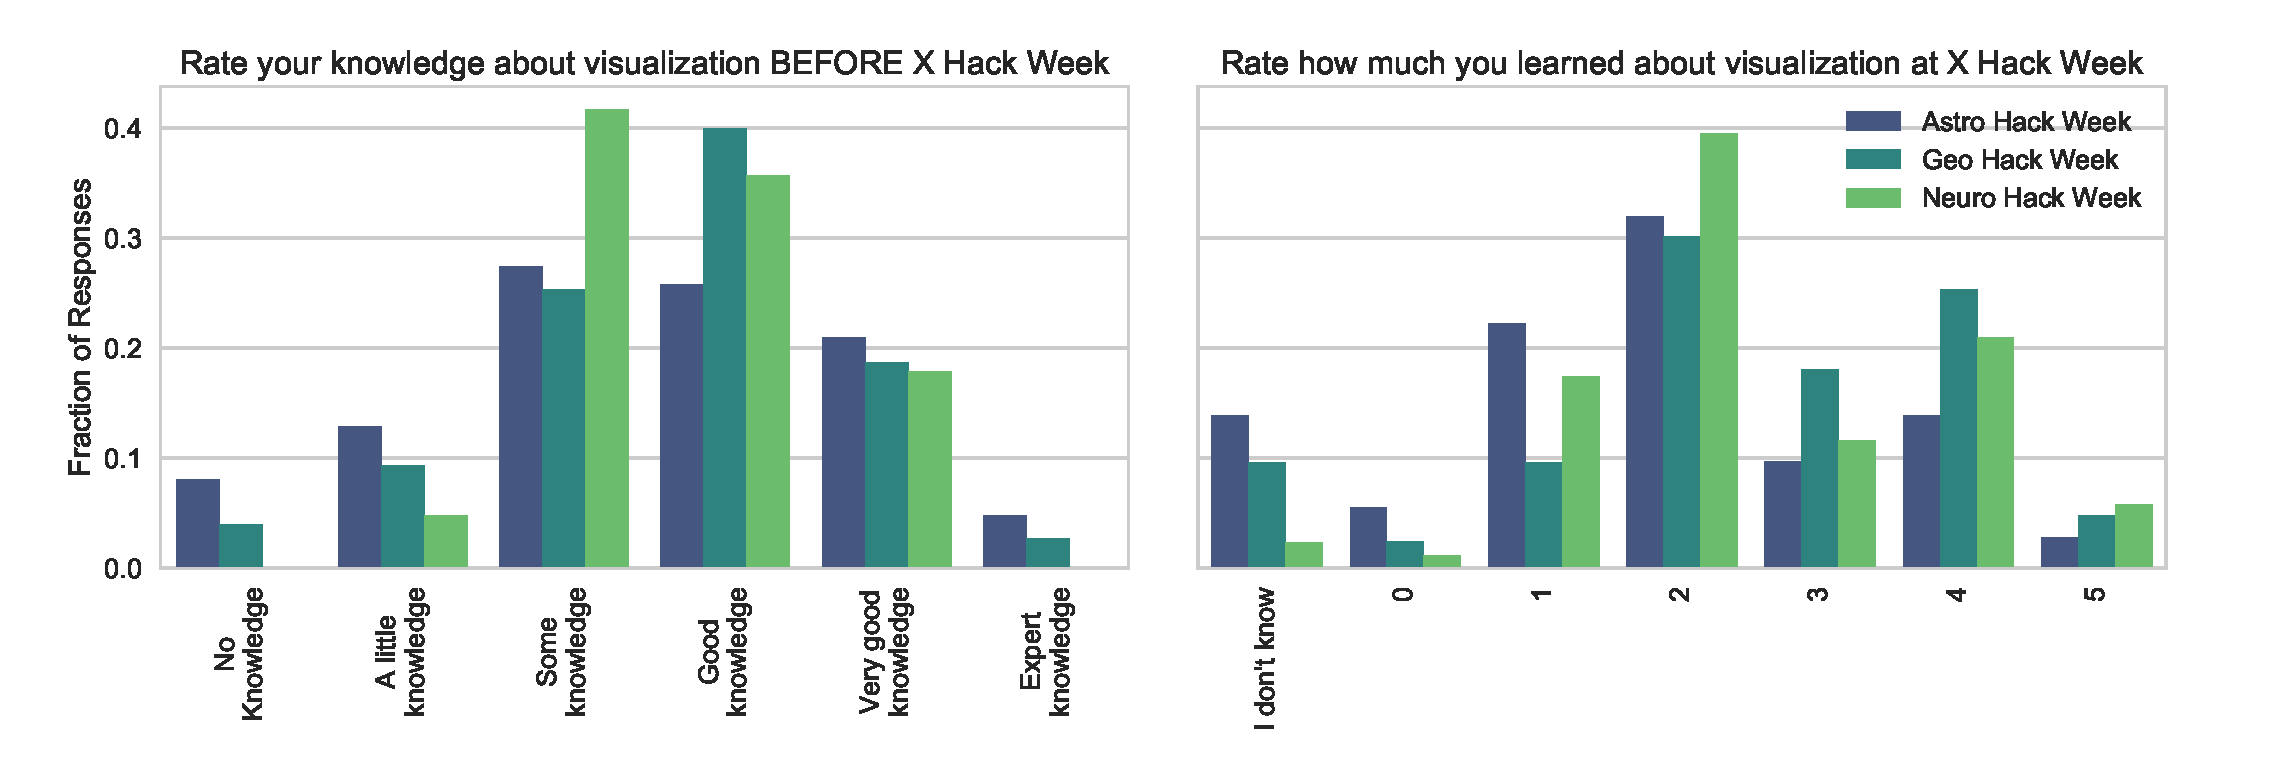
\includegraphics[width=11cm]{fig/longitudinal_visualization.eps}
\end{subfigure}

\begin{subfigure}[t]{\textwidth}
\centering
\caption{}
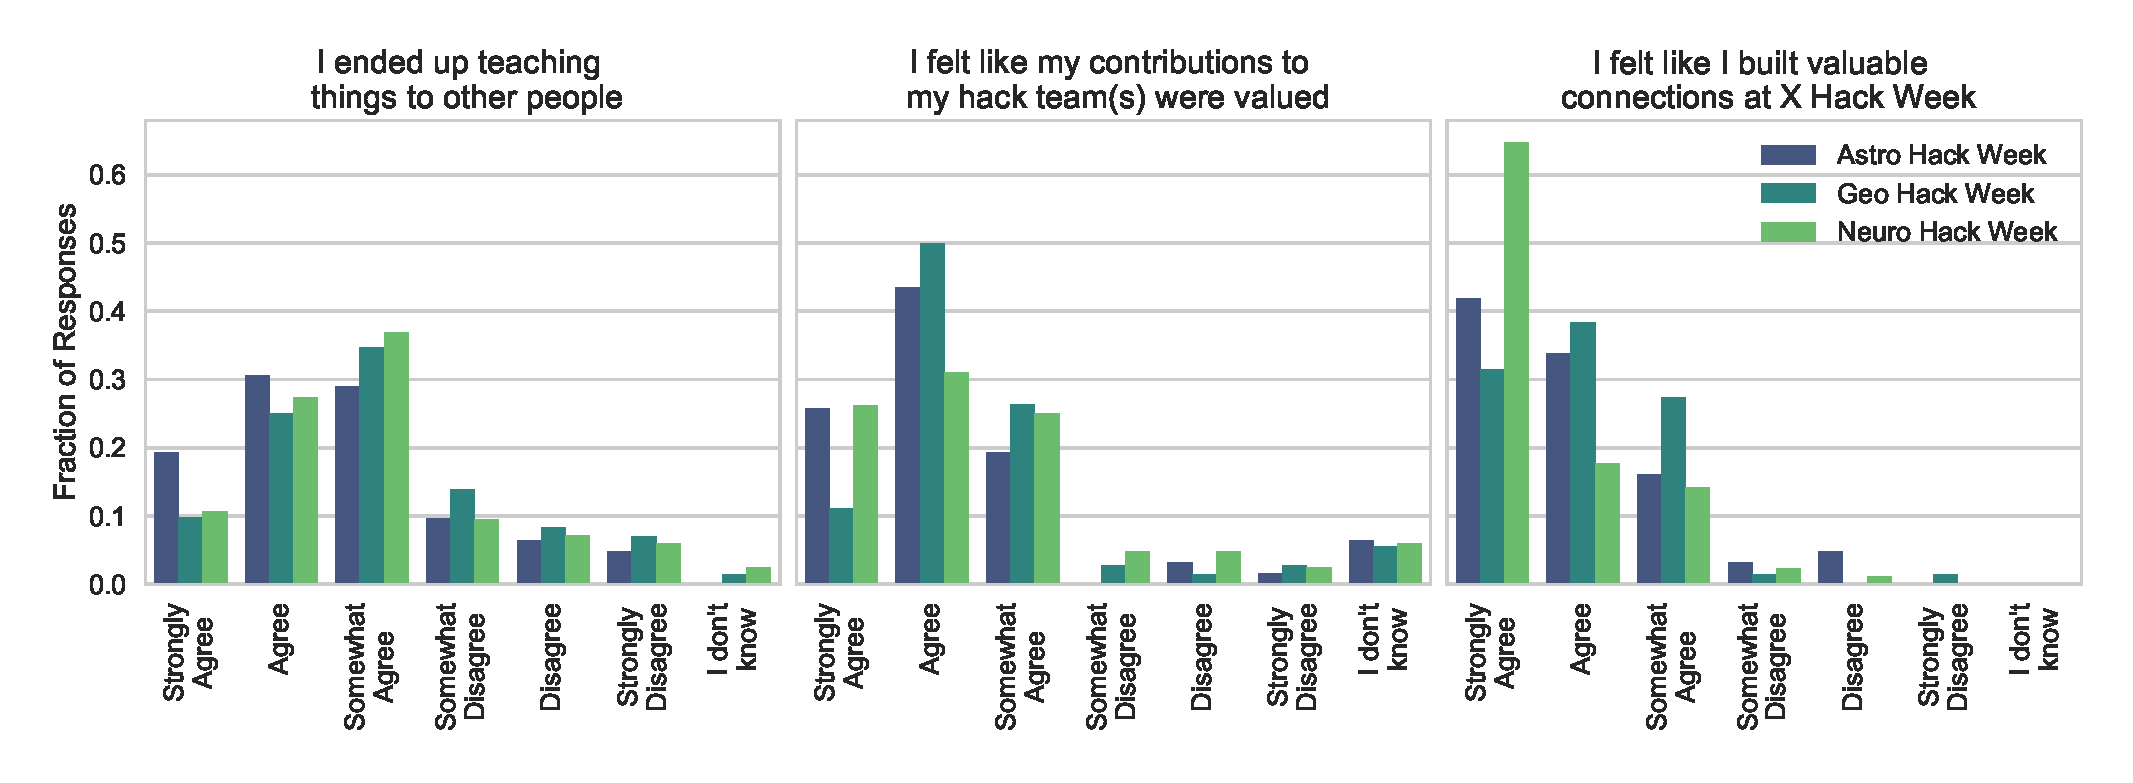
\includegraphics[width=11cm]{fig/eval_collab.eps}
\end{subfigure}

\begin{subfigure}[t]{\textwidth}
\centering
\caption{}
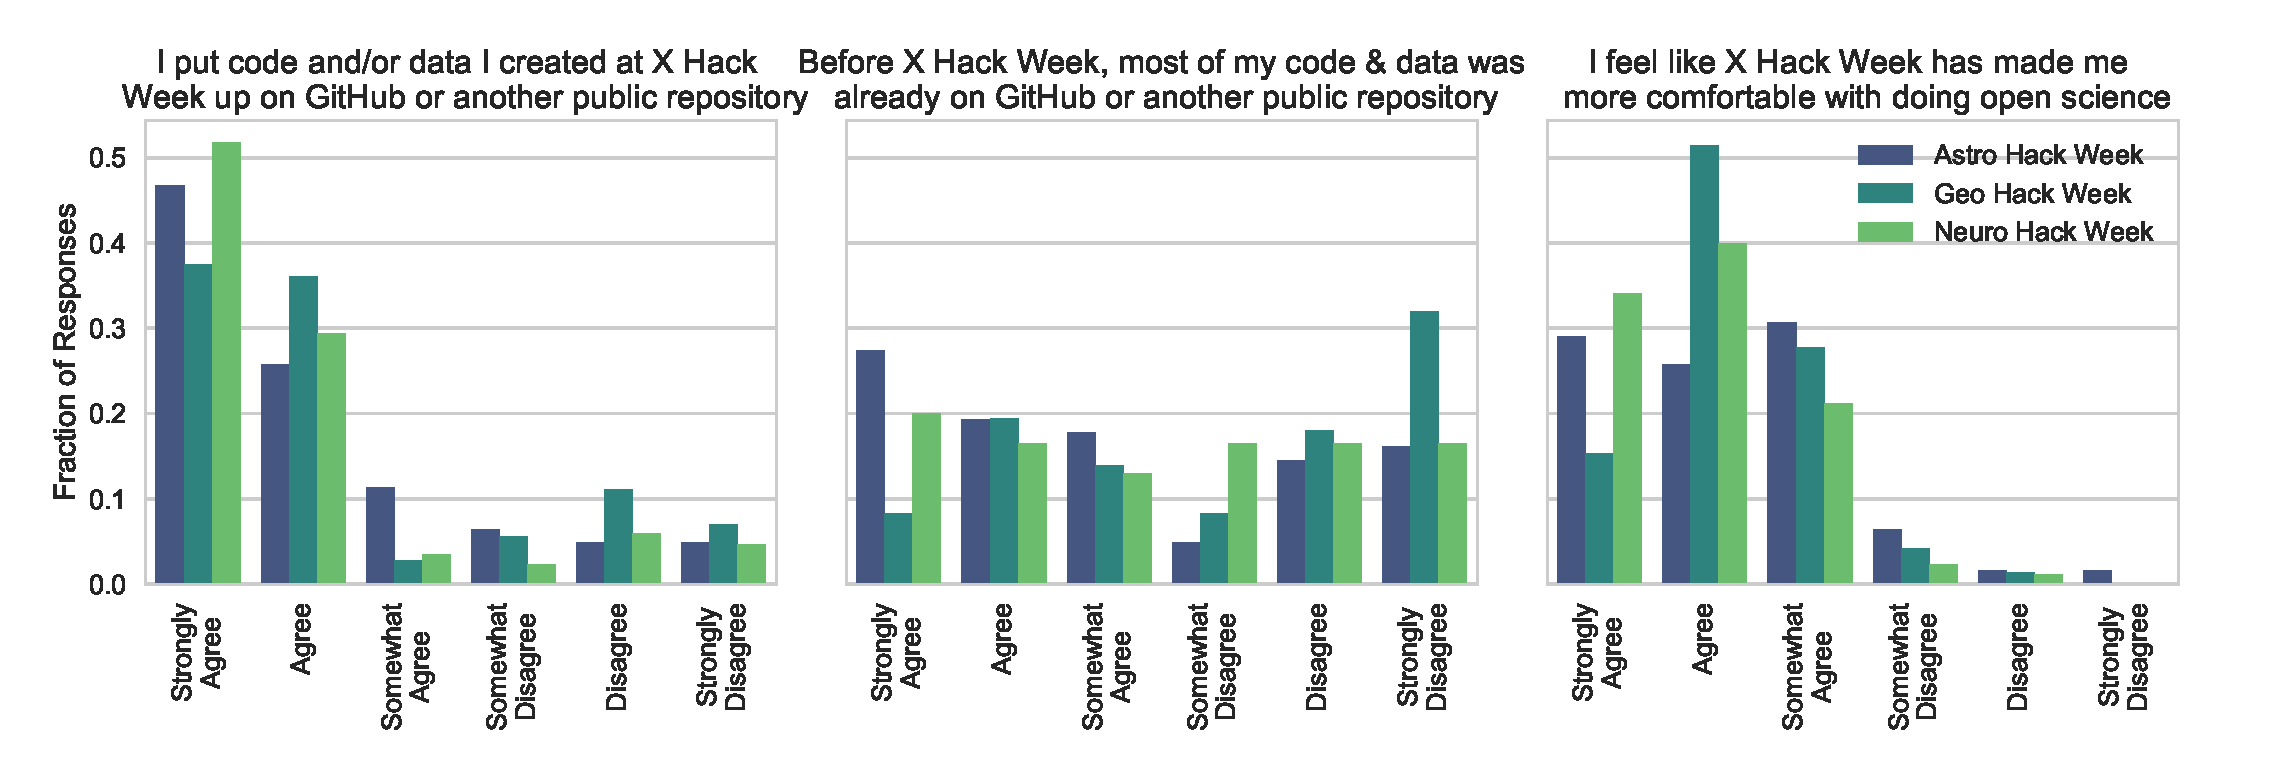
\includegraphics[width=11cm]{fig/eval_openscience.eps}
\end{subfigure}

\caption{{\bf Post-workshop surveys from three hack weeks}: participants in the 2016 astro-, geo- and neuro- hack weeks responded to questions assessing their experiences. \textbf{For GHW and NHW, response rates were 100\%, with $N_{\mathrm{GHW}}= 83$ and $N_{\mathrm{NHW}} = 86$, respectively. At AHW, the combined response rate for both years was 76\%, or $N_{\mathrm{AHW}} = 72$ out of $94$ total attendees. We report here about results in three different domains: the development of technical skills (a and b), collaboration and learning (c), and shifts in attitudes towards reproducibility and open science (d)}}
\label{fig:survey}
%\end{center}
\end{figure*}

Measuring the success of a hack week objectively is complicated by the variety of objectives that a hack week might have (see above). 
Additionally, the participant-driven, open-ended format facilitates knowledge transfer and collaborations in sometimes surprising ways that escape traditional measures of success.

One key metric is the number of publications that result from hack week projects, but this is a fairly narrow definition of success, in line with standard academic performance indicators.
Assuming that participants work largely in the open during a hack week, and that most projects have a strong programming component another indicator of success is the activity of participants in terms of code written and committed to a public code repository.
Still, these measures ignore learning, community-building as well as networking outcomes, which can be assessed through post-workshop surveys.
%It is in principle possible to measure gains in knowledge, networks and productivity within the pool of acceptable candidates for both those that attended the hack week and those that did not.
%This would then provide a somewhat objective measure of the impact the hack week has had.
%In practice, this has not been done for any of the hack weeks conducted thus far.
Here, we have taken an approach that combines these metrics: we start with survey results, and anecdotally report about publications, new code and projects generated (see the following section).
%Open-ended questions allow participants to provide feedback about outcomes, problems and goals that organizers had not anticipated.

%If hack week organizers plan to conduct research that involves hack week participants (for example, using assessments and evaluations in a paper such as this one) it is important to obtain approval from the Institutional Review Board (IRB), or equivalent body that approves research with human participants at the institution hosting the hack week.
%Though this research would usually fall under the category of ''minimal risk``, it is still important to establish procedures to manage these data, and to obtain informed consent.
%In particular, in some cases hack week organizers may be interested in studying not only the participants in the hack week, but also the applicants who did not end up participating.
%It is important to establish procedures to conduct such studies and to obtain approval from an IRB.

Focusing on the outcomes of astro-, geo- and neuro- hack weeks (AHW, GHW, NHW, respectively) from 2016, we find that \textbf{most} participants self-report successful learning outcomes.  in new topics, tools or methods (AHW: 76\%, GHW: 89\%, NHW: 79\% for responses ``somewhat agree'', ``agree'' and ``strongly agree''; Figure \ref{fig:survey}, (a), left).
The overwhelming majority of respondents at the hack weeks ($>95\%$ for all three events) believed that they learned things that improve their day-to-day research, and that attendance has made them a better scientist (Figure \ref{fig:survey}, (a), right and middle).
\textbf{More specifically, we compared learning outcomes in data visualization (the only topic explicitly shared between all three hack weeks; Figure \ref{fig:survey}, (b), left). We asked participants to subjectively rate their knowledge before the hack week, and find skill levels to be broadly distributed. This is expected, given the goal of diversity during the selection stage, but we also note that there might be systematic effects, since the way the question was posed may be subject to individual biases. We then asked participants to rate their learning outcomes at the hack weeks in this category, and find that most participants have positive learning outcomes at all three hack weeks for data visualization, but that outcomes vary strongly, as is expected, too, with a group that is this diverse \textit{a priori}.}
%While each hack week also probed participants' attitudes in more detail toward specific topics, methods, and modes of learning, the hack weeks differed substantially on that level, making the results difficult to compare.
%Another important goal of the hack weeks was centred on community building and fostering collaborations.
The majority of participants felt that their contributions to their hack teams was valued, and that they built valuable connections to other researchers (Figure \ref{fig:survey}, middle panel, middle).
This is especially true for Neuro Hack Week, where more than 64\% of participants strongly agreed that they formed valuable connections at NHW (Figure  \ref{fig:survey}, middle panel, right).
Because peer learning is a major mode of knowledge transfer at hack weeks, we asked participants whether they taught other participants.
We find that again a majority agrees with this statement to some degree (AHW: 79\%, GHW: 69\%, NHW: 75\% for combined responses ``somewhat agree'', ``agree'' and ``strongly agree''; Figure \ref{fig:survey}, middle panel, left), though responses are not as unequivocal as they are in some of the other categories.
This is expected: participants new to the field may participate to learn rather than to teach. \textbf{It is notable, however, that we find no correlation between the response to this question and career stage for any of the events surveyed here. In particular, participants from all career stages between graduate students and tenured faculty report similar engagement in teaching. This supports our hypothesis that compared to e.g.\ a traditional summer school, a hack week is less hierarchical and encourages lateral knowledge transfer between participants at different career stages.  We similar find no correlations with gender identity or race/ethnicity. Responses to the other two questions regarding whether participants' contributions to hack teams were valued and whether they made valuable connections at the hack week were similarly evenly distributed across career stages, gender and racial/ethnic identities.}

We find that the hack weeks have been largely successful at efforts to promote positive attitudes towards reproducibility and open science: at all three events, more than 85\% of all participants (AHW: 86\%, GHW: 94\%, NHW: 95\%; Figure \ref{fig:survey}, bottom panel, left) put code or data created at the hack week into a public repository, while a substantially smaller fraction of participants followed this practice before the event (Figure \ref{fig:survey}, bottom panel, middle).
When asking participants whether they had made their code or data openly available in the past, the overall behaviour reflects how general conventions and attitudes differ in different fields.
Astronomy shows the largest degree of openness toward open science, whereas our results indicate that open science is still fairly uncommon in the geosciences, with neuroscience falling in between.
%This implies that hack weeks can have the highest impacts in field where a priori engagement in reproducibility efforts is low and significant progress can be made towards changing researchers' attitudes during a collaborative workshop.
Similar attitudes are reflected when asking whether the hack week has made participants more comfortable with open science: again, geoscience shows the large improvement with over 97\% agreeing with this statement to some degree, closely followed by neuroscience (95\%), while there was somewhat less of an impact on participants' attitudes in astronomy (72\%).
Overall, our results show that hack weeks are effective at addressing persisting doubts about making research open and reproducible. \textbf{While the focus on open science is not necessarily a required component of a hack week, it aligns naturally with many of the goals and values commonly promoted at hack weeks, including open-source software, data sharing and reproducibility. In some fields, especially where ethical issues around data sharing and privacy are relevant, this might not be a desired focus of the hack week, or might be replaced or augmented by a discussion of ethical considerations.}

From the very nature of the activities that we encourage in hack weeks, participants in these events produce digital records of their research online. This means that it will be fairly straightforward to evaluate the long-term impact of these activities on participants' productivity (e.g., through contributions to open-source software) in the future. Because all three events are relatively recent, it is still early to evaluate such long-term outcomes, as well as others including publications and collaborations resulting from these events.
There are, however, initial indicators that all hack weeks encouraged long-term engagement with new concepts or tools and that they directly resulted in a number of publications \cite{gullysantiago2015,faria2016,keshavan2017,leonard2017,jordan2017,peterson2017,hahn2017,pricewhelan2017}. For specific examples, see also below.

\subsection*{Examples of Hack Week Outcomes}
\label{sec:outcomes}
\subsubsection*{Example 1: Astro Hack Week}
In 2015, a small team used the opportunity of AHW to found a new software project called Stingray\footnote{https://github.com/StingraySoftware/stingray} with the goal of providing well-tested, well-documented implementations of time series analysis algorithms often used in X-ray astronomy.
The start of this project was facilitated by the collaborative environment at Astro Hack Week, including expertise in how to start/run open-source projects, role models of successful projects, and an environment encouraging scientific risk taking. Astro Hack Week enabled participants to seed a new collaboration around a software project needed by the larger community.
Since its beginnings at Astro Hack Week, Stingray has matured into an enduring collaboration within the community with five active maintainers, a number of contributors and four Google Summer of Code projects.
\subsubsection*{Example 2: Geo Hack Week}
In 2016, a GHW project team used Google Earth Engine to explore spatial patterns in climate, topography and population data with the goal of mapping the most suitable locations for renewable energy sites in the United States.
The team used machine learning algorithms in conjunction with the powerful hardware resources provided by Google Earth Engine\footnote{\url{http://georgerichardson.net/2017/04/10/searching-for-energy-in-a-random-forest/}}.
George Richardson, one of the project leads, now works for a renewable resource company in Seattle.
\subsubsection*{Example 3: Neuro Hack Week}
Motion of study participants inside of the MRI machine is a major concern in neuroimaging studies, particularly in studies of children or patients, as they are more likely to move.
During NHW 2016 one of the teams focused on a large and openly available data-set of MRI data from children\footnote{ABIDE: \url{http://preprocessed-connectomes-project.org/abide}}.
To test the effect of motion on the results, the team conducted an analysis in which both the number of experimental subjects included, as well as motion cut-off were varied.
%They tested both the split-half reliability of an analysis of brain connectivity, as well as an analysis that used machine learning to distinguish between brains of children with and without autism spectrum disorder.
The team (composed of four different researchers from four different institutions in two different countries) continued to work on this project remotely after the end of Neuro Hack Week, and eventually published a paper describing these results in the open access journal Research Ideas and Outcomes \cite{leonard2017}.


\section*{Conclusions}

The fast-paced changes of the computational and methodological landscape require traditional fields of science to rapidly adapt to new data analysis challenges.
Traditional modes of learning, including university curricula, are often too slow to incorporate new developments on short enough time scales to meet their acute need in scientific advancement.
To address this imbalance, new types of workshops, including unconferences, hackathons and bootcamps, have been developed in recent years in various scientific disciplines to exist alongside with and support the existing structure of academic conferences.
Here, we introduce one such concept, hack weeks, and detail the underlying philosophical ideas along with experiences from events held in three different fields

As introduced above, hack weeks serve multiple purposes, including dissemination of state-of-the-art technological advances through the scientific community, building collaborations between academic subdisciplines and fostering interdisciplinary research as well as  promoting open science and reproducibility.
Initial results from three events held in 2016 and 2017 in three different fields (astronomy, geosciences and neurosciences) indicate that hack weeks succeed at all of these objectives, but that the measure of success is field-specific in that it depends to some degree on how much the concepts hack weeks promote were already adopted within the community.
Hack weeks are still a very young concept, and estimating the long-term impact of these events within the scientific communities they serve will require follow-up over multiple years to asses their effect on collaboration networks, career outcomes for early-career academics and adoption of new methods.
We have shown, however, that hack weeks provide an easy-to-implement, fairly low-cost method to introduce new technologies and methods into scientific fields on much shorter time scales than traditional teaching efforts can.
While we focus here on hack weeks in scientific fields, the concept could be extended to other areas, and is more generally useful in any area (1) where useful tools can be learned in short tutorials, (2) where results and outcomes can be produced on the timescale of a few days, and (3) that would benefit from collaborative approaches that cross traditional boundaries. Such areas could include for example the social sciences, music and art.


%Spelling must be British English (Oxford English Dictionary)

%In addition, a cover letter needs to be written with the
%following:
%\begin{enumerate}
% \item A 100 word or less summary indicating on scientific grounds
%why the paper should be considered for a wide-ranging journal like
%\textsl{Nature} instead of a more narrowly focussed journal.
% \item A 100 word or less summary aimed at a non-scientific audience,
%written at the level of a national newspaper.  It may be used for
%\textsl{Nature}'s press release or other general publicity.
% \item The cover letter should state clearly what is included as the
%submission, including number of figures, supporting manuscripts
%and any Supplementary Information (specifying number of items and
%format).
% \item The cover letter should also state the number of
%words of text in the paper; the number of figures and parts of
%figures (for example, 4 figures, comprising 16 separate panels in
%total); a rough estimate of the desired final size of figures in
%terms of number of pages; and a full current postal address,
%telephone and fax numbers, and current e-mail address.
%\end{enumerate}

%See \textsl{Nature}'s website
%(\texttt{http://www.nature.com/nature/submit/gta/index.html}) for
%complete submission guidelines.

%\begin{methods}
%Put methods in here.  If you are going to subsection it, use
%\verb|\subsection| commands.  Methods section should be less than
%800 words and if it is less than 200 words, it can be incorporated
%into the main text.


%\end{methods}

%% Put the bibliography here, most people will use BiBTeX in
%% which case the environment below should be replaced with
%% the \bibliography{} command.

% \begin{thebibliography}{1}
% \bibitem{dummy} Articles are restricted to 50 references, Letters
% to 30.
% \bibitem{dummyb} No compound references -- only one source per
% reference.
% \end{thebibliography}

\section{References}
\bibliographystyle{naturemag}
\bibliography{paper}


%% Here is the endmatter stuff: Supplementary Info, etc.
%% Use \item's to separate, default label is "Acknowledgements"

\begin{addendum}
 \item{The authors would like to thank Laura Nor\'{e}n (NYU) for help on ethics and IRB, Stuart Geiger for helping to formulate the questionnaires that served as the basis for the results presented here. This work was partially supported by the Moore-Sloan Data Science Environments at UC Berkeley, New York University, and the University of Washington. Neurohack week is supported through a grant from the National Institute for Mental Health (1R25MH112480). Daniela Huppenkothen is partially supported by the James Arthur Postdoctoral Fellowship at NYU.}
 \item[Competing Interests]{The authors declare that they have no competing financial interests.}
 \item[Correspondence]{Correspondence and requests for materials should be addressed to D.Huppenkothen.~(email: daniela.huppenkothen@nyu.edu).}
\end{addendum}

%%
%% TABLES
%%
%% If there are any tables, put them here.
%%

%\begin{table}
%\centering
%\caption{This is a table with scientific results.}
%\medskip
%\begin{tabular}{ccccc}
%\hline
%1 & 2 & 3 & 4 & 5\\
%\hline
%aaa & bbb & ccc & ddd & eee\\
%aaaa & bbbb & cccc & dddd & eeee\\
%aaaaa & bbbbb & ccccc & ddddd & eeeee\\
%aaaaaa & bbbbbb & cccccc & dddddd & eeeeee\\
%1.000 & 2.000 & 3.000 & 4.000 & 5.000\\
%\hline
%\end{tabular}
%\end{table}

\end{document}
